\chapter{Influence of non-axisymmetric planetary field on Jupiter's magnetosphere and current sheet}

\section{Jupiter's oscillating current sheet}

\begin{figure}
    \centering
    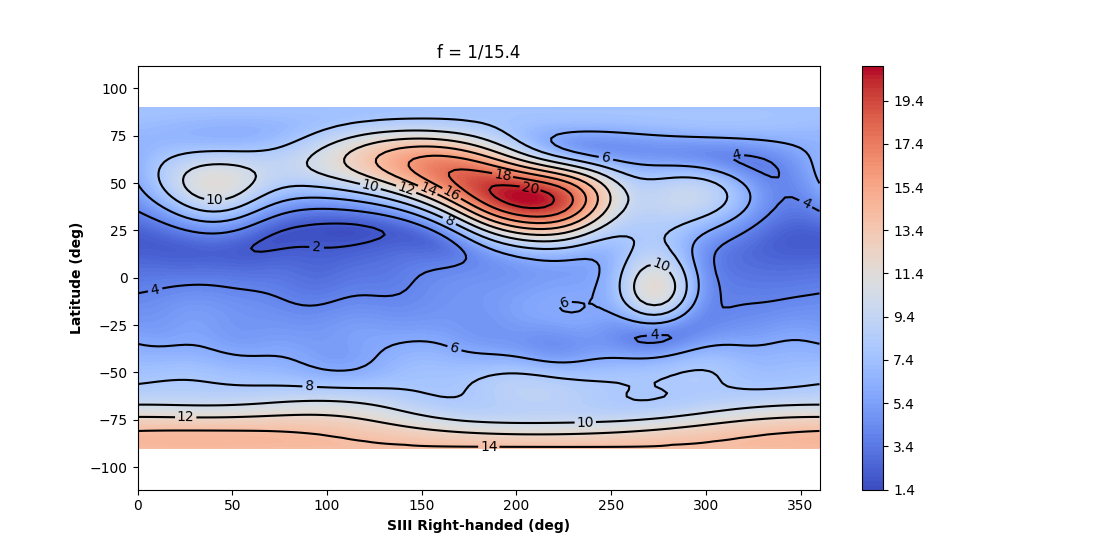
\includegraphics[width=\textwidth]{images6/JRM09_Bmag.png}
    \caption{Contours of the magnetic field strength (in Gauss) on the 1 bar surface of Jupiter as per the JRM09 magnetic field model \protect\cite{Connerney2018}.}
    \label{fig:JRM09}
\end{figure}

by Pioneer 10, Pioneer 11, Voyager 1, Voyager 2, Galileo and Juno

\begin{figure}
    \centering
    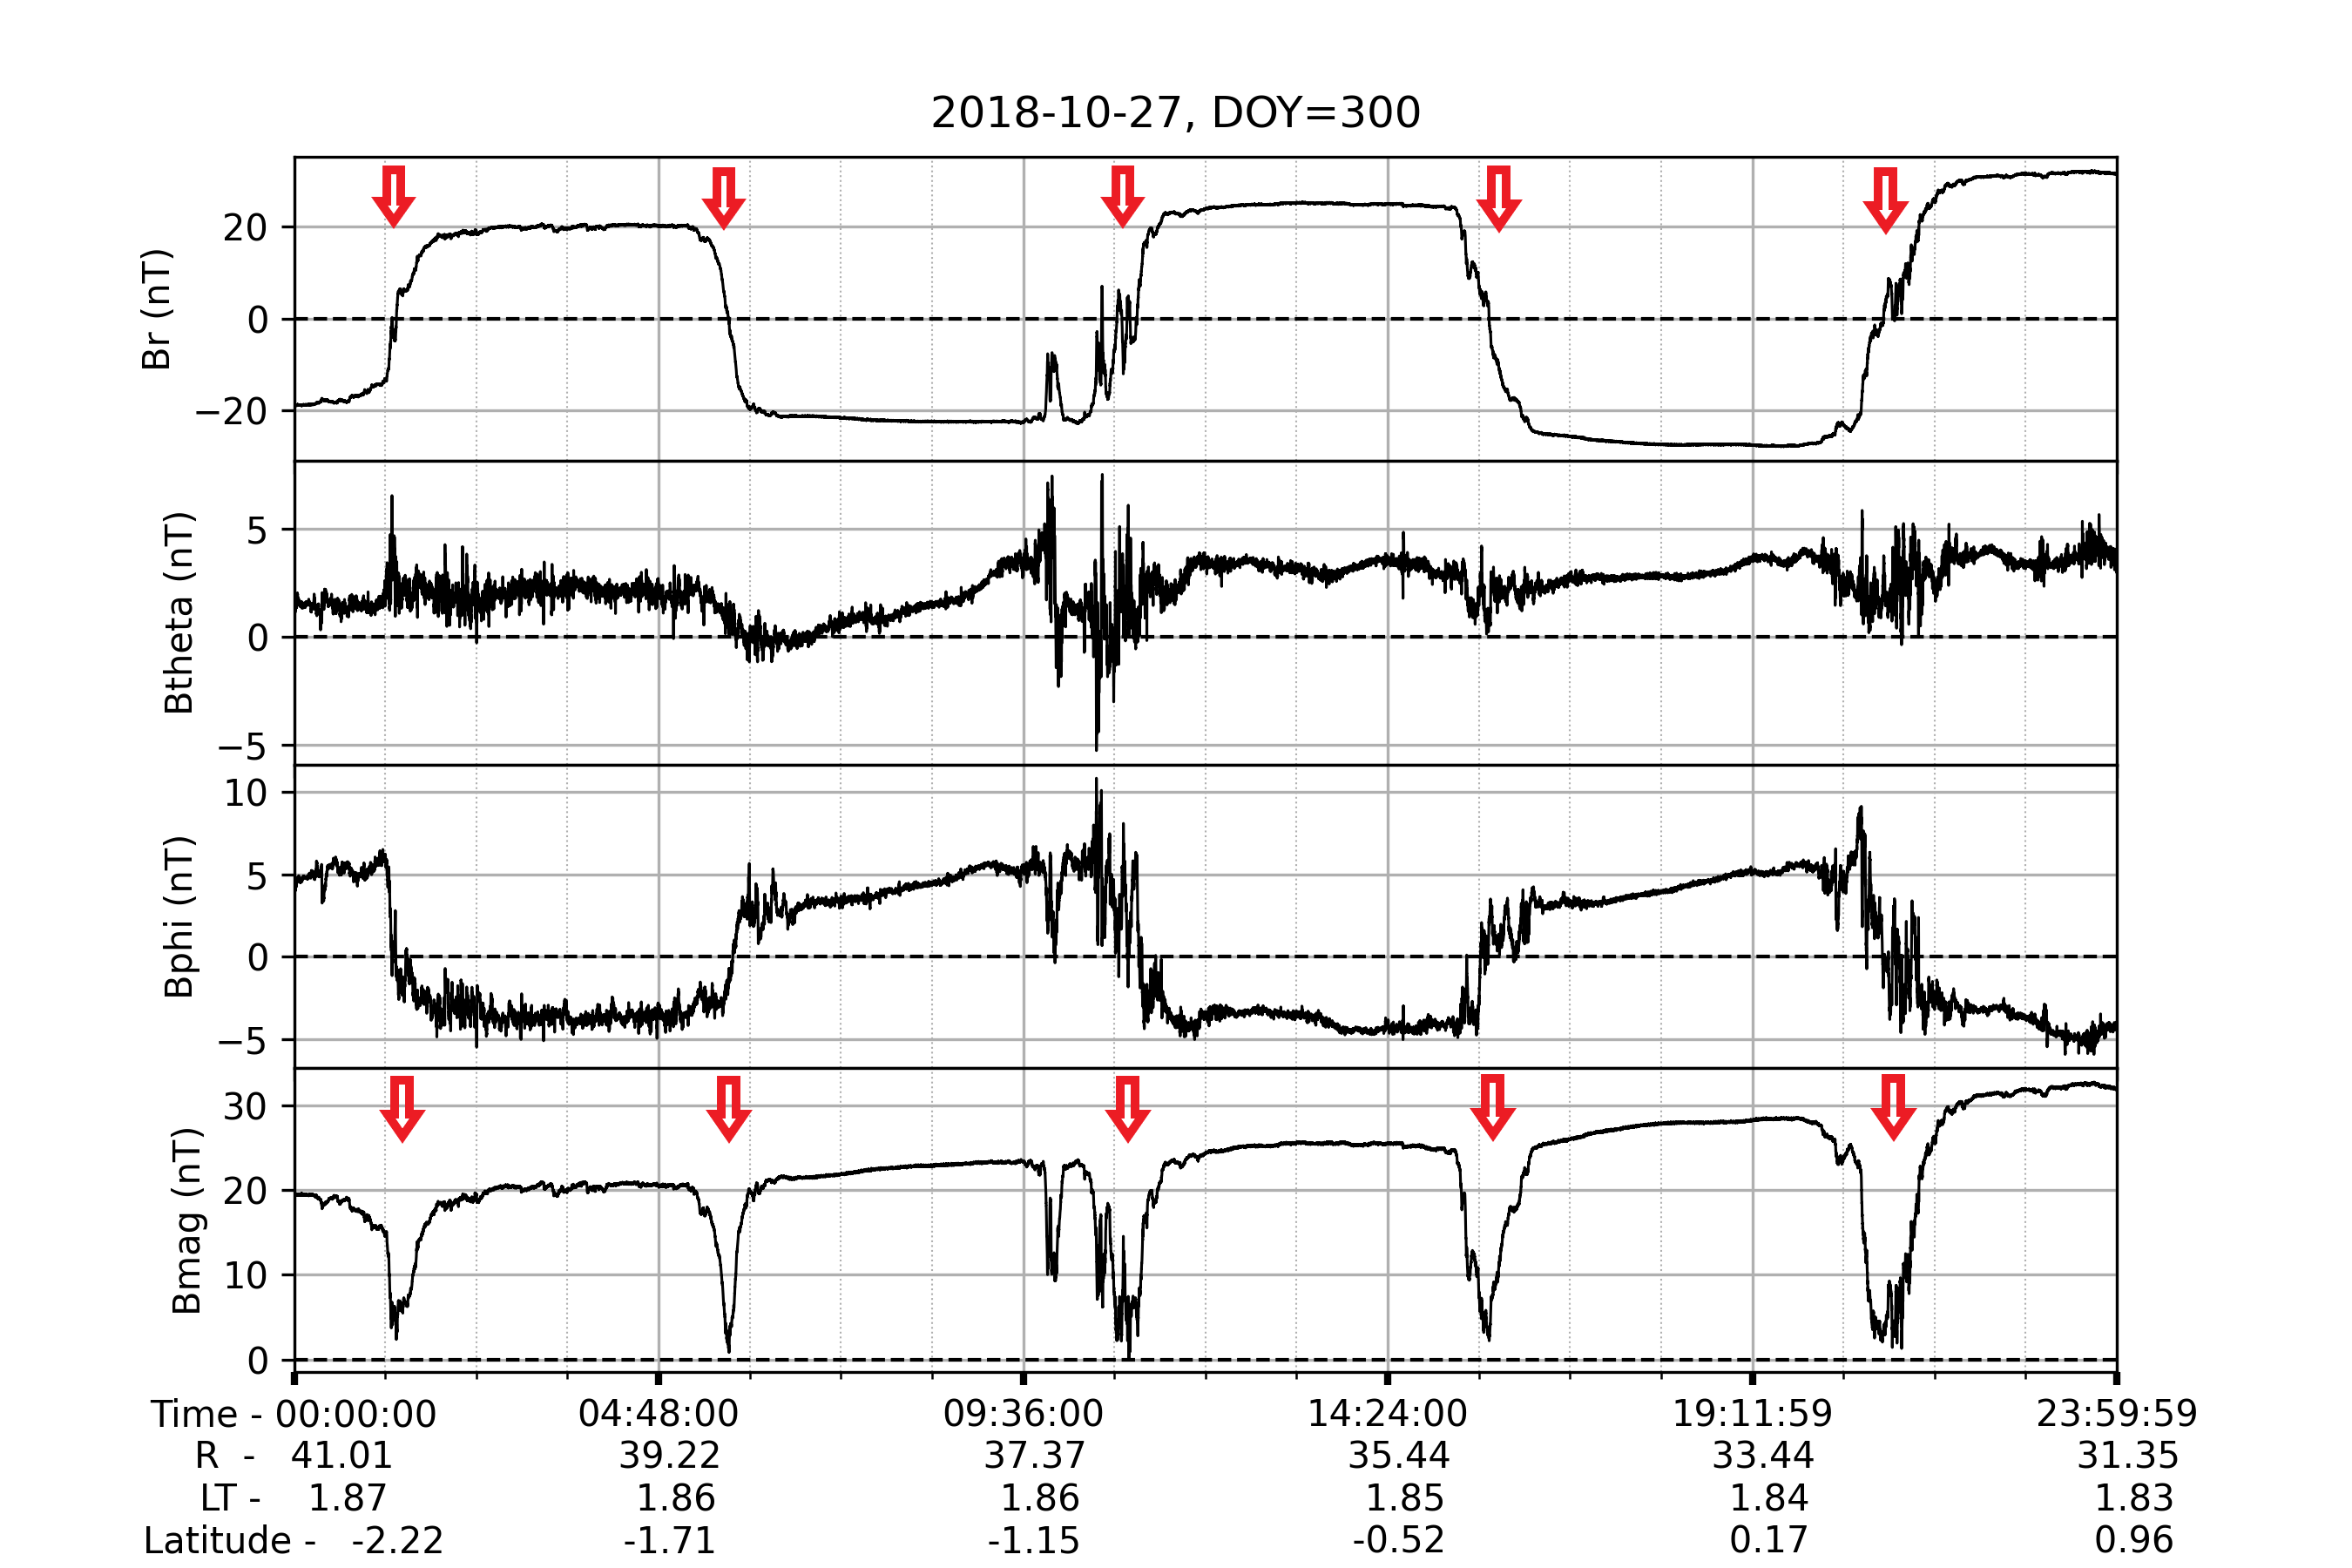
\includegraphics[width=\textwidth]{images6/Juno-currentsheet-observations.png}
    \caption{Magnetic field measurements taken by the Juno spacecraft in the JSS coordinate system ($B_r$, $B_\theta$, $B_\phi$, $|B|$). Juno crosses the current sheet twice every rotation period, as seen in the multiple reversals of $B_r$ separated by roughly $\sim$5 hours.}
    \label{fig:juno-current-sheet}
\end{figure}

Many empirical models have been put forward to account for the variation of the Jovian current sheet due to the non-axisymmetric internal field. Each model has a different set of parameters which are varied to minimize the $\chi^2$ error between the modeled current sheet location and that seen in-situ by the relevant spacecraft. Although they can be used to infer the location of the current sheet, these models do not provide any information about its strength. They can be categorized into two classes, which are discussed below. 

\subsection{Axial models}
Initial models assumed that the Jovian current sheet would be located in a plane corresponding to the magnetic equator of Jupiter, which would rotate at the planetary rotation period. The expected $z$ location of the current sheet at a given radial location in cylindrical coordinates $(\rho, \phi)$ could then be described simply as \cite{VanAllen1974EnergeticJupiter,Goertz1976TheMagnetosphere},

\begin{equation}
    z = -\rho \tan\theta_d \cos\left(\phi - \phi_d\right)
\end{equation}

Where $\theta_d$ is the tilt of the assumed planetary dipole field with respect to the rotation axis and $\phi_d$ provides the azimuthal location of the magnetic North pole. The rigid tilted plane model was found to be inaccurate at large distances, and the model was modified to limit the $z$ excursions of the current sheet at large radial distances. The first \emph{hinged} current sheet models \cite{Smith1974The10,Hill1974ConfigurationMagnetosphere} simply added a condition to limit these excursions $\rho > a$, where $a$ is the hinging distance and is the only free parameter.
\begin{equation}
    z = \begin{cases}
    -\rho \tan\theta_d \cos\left(\phi - \phi_d\right), & \text{for } \rho \leq a\\
    -a \tan\theta_d \cos\left(\phi - \phi_d\right), & \text{for } \rho > a
    \end{cases}
\end{equation}

Or alternatively, using a $\tanh$ function, 
\begin{equation}
    z = -a \tanh\left(\frac{\rho}{a}\right) \tan\theta_d \cos\left(\phi - \phi_d\right)
\end{equation}

An improvement was suggested by \citeA{Kivelson1978ASheet} to add a phase delay to the current sheet location, proportional to the distance from the wave source and has the following functional form,
\begin{equation}
    \phi' = \phi_d - \frac{\Omega \left( \rho - \rho_0\right)}{U}
\end{equation}

Where $\Omega$ is the angular velocity of Jupiter, $U$ is the speed at which the wave travels and $\rho_0$ serves as the radial distance where the current sheet ceases to follow the rotating plane, beyond which all locations perceive a delay in the arrival of the current sheet. The expected current sheet location in the \citeA{Kivelson1978ASheet} model is then given by,
\begin{equation}
    z = \begin{cases}
    -\rho \tan\theta_d \cos\left(\phi - \phi_d\right), & \text{for } \rho < \rho_0\\
    -\rho \tan\theta_d \cos\left(\phi - \phi'\right),  & \text{for } \rho \geq \rho_0
    \end{cases}
    \label{eqn:kivelson1978}
\end{equation}

\citeA{Eviatar1976PlasmaMagnetosphere} introduced a similar model but limited the latitudinal extent of the oscillation beyond $\rho \geq \rho_0$,
\begin{equation}
    z = \begin{cases}
    -\rho \tan\theta_d \cos\left(\phi - \phi_d\right), & \text{for } \rho < \rho_0\\
    -a \tan\theta_d \cos\left(\phi - \phi'\right),  & \text{for } \rho \geq \rho_0
    \end{cases}
\end{equation}

Lastly, \citeA{Behannon1981} introduced another axial model which included the effects of wave propagation and current sheet hinging (Equation 11 in \citeA{Behannon1981}). However, they assume that the wave starts propagating from the origin $\rho_0=0$.
\begin{equation}
    z = -a \tanh\left(\frac{\rho}{a}\right) \tan\theta_d \cos\left(\phi - \phi_d + \frac{\Omega \rho}{U}\right)
    \label{eqn:behannon1981}
\end{equation}

\subsection{Non-axial models}
Axial models were found to fit the data poorly at large distances in the magnetotail, and it was suggested that the interaction of the magnetosphere with the solar wind may lead to a formation of a magnetotail, where the current sheet would take the form of a rocking plane. The rocking plane model does not accurately represent the current sheet near the planet. \citeA{Behannon1981} suggested a hybrid model which follows the magnetic equator close to the planet and take the form of a rocking plane at large distances (also called the Rocking Plane/Rotating Disk model or RP/RD).

\begin{equation}
    \phi' = \phi_d - \frac{\Omega \left(x - a\right)}{U}
\end{equation}
\begin{equation}
    z = x \sech \left( \frac{x}{a} \right) \cos\left(\phi - \phi' \right) + y \sin\left(\phi - \phi' \right)  
\end{equation}

Note that the above model follows a rotating disk near the planet where $\phi'=\phi_d$. The wave starts propagating at distance $a$ at a fixed speed $U$, which are the two parameters for this model. \citeA{Khurana1992ASheet} extend the previous models by prescribing a variation in the wave propagation speed with radial distance as follows,

\begin{equation}
    v(\rho) = v_0 \coth \left(\frac{\rho}{\rho_0} \right)
\end{equation}
which leads to the following expressions for the phase delay and the current sheet location,
\begin{equation}
    \phi' = \phi_d - \Omega \int \frac{d\rho}{v(\rho)} = \phi_d - \frac{\Omega \rho}{v_0} \ln \cosh \left( \frac{\rho}{\rho_0} \right) 
\end{equation}
\begin{equation}
    z = -\rho \tan\theta_d \cdot \frac{x_0}{x} \tanh\left(\frac{x}{x_0} \right) \cos\left( \phi - \phi'\right) 
    \label{eqn:khurana1992}
\end{equation}
The \citeA{Khurana1992ASheet} model has three parameters $(v_0, \rho_0, x_0)$ representing the asymptotic wave propagation speed, radial location of outflow, and the hinging point along the X-axis. \citeA{Khurana2005} updated the model to account for local time asymmetries and solar wind angle of attack, but the generalization increases the number of parameters in the model. 

\begin{figure}
    \centering
    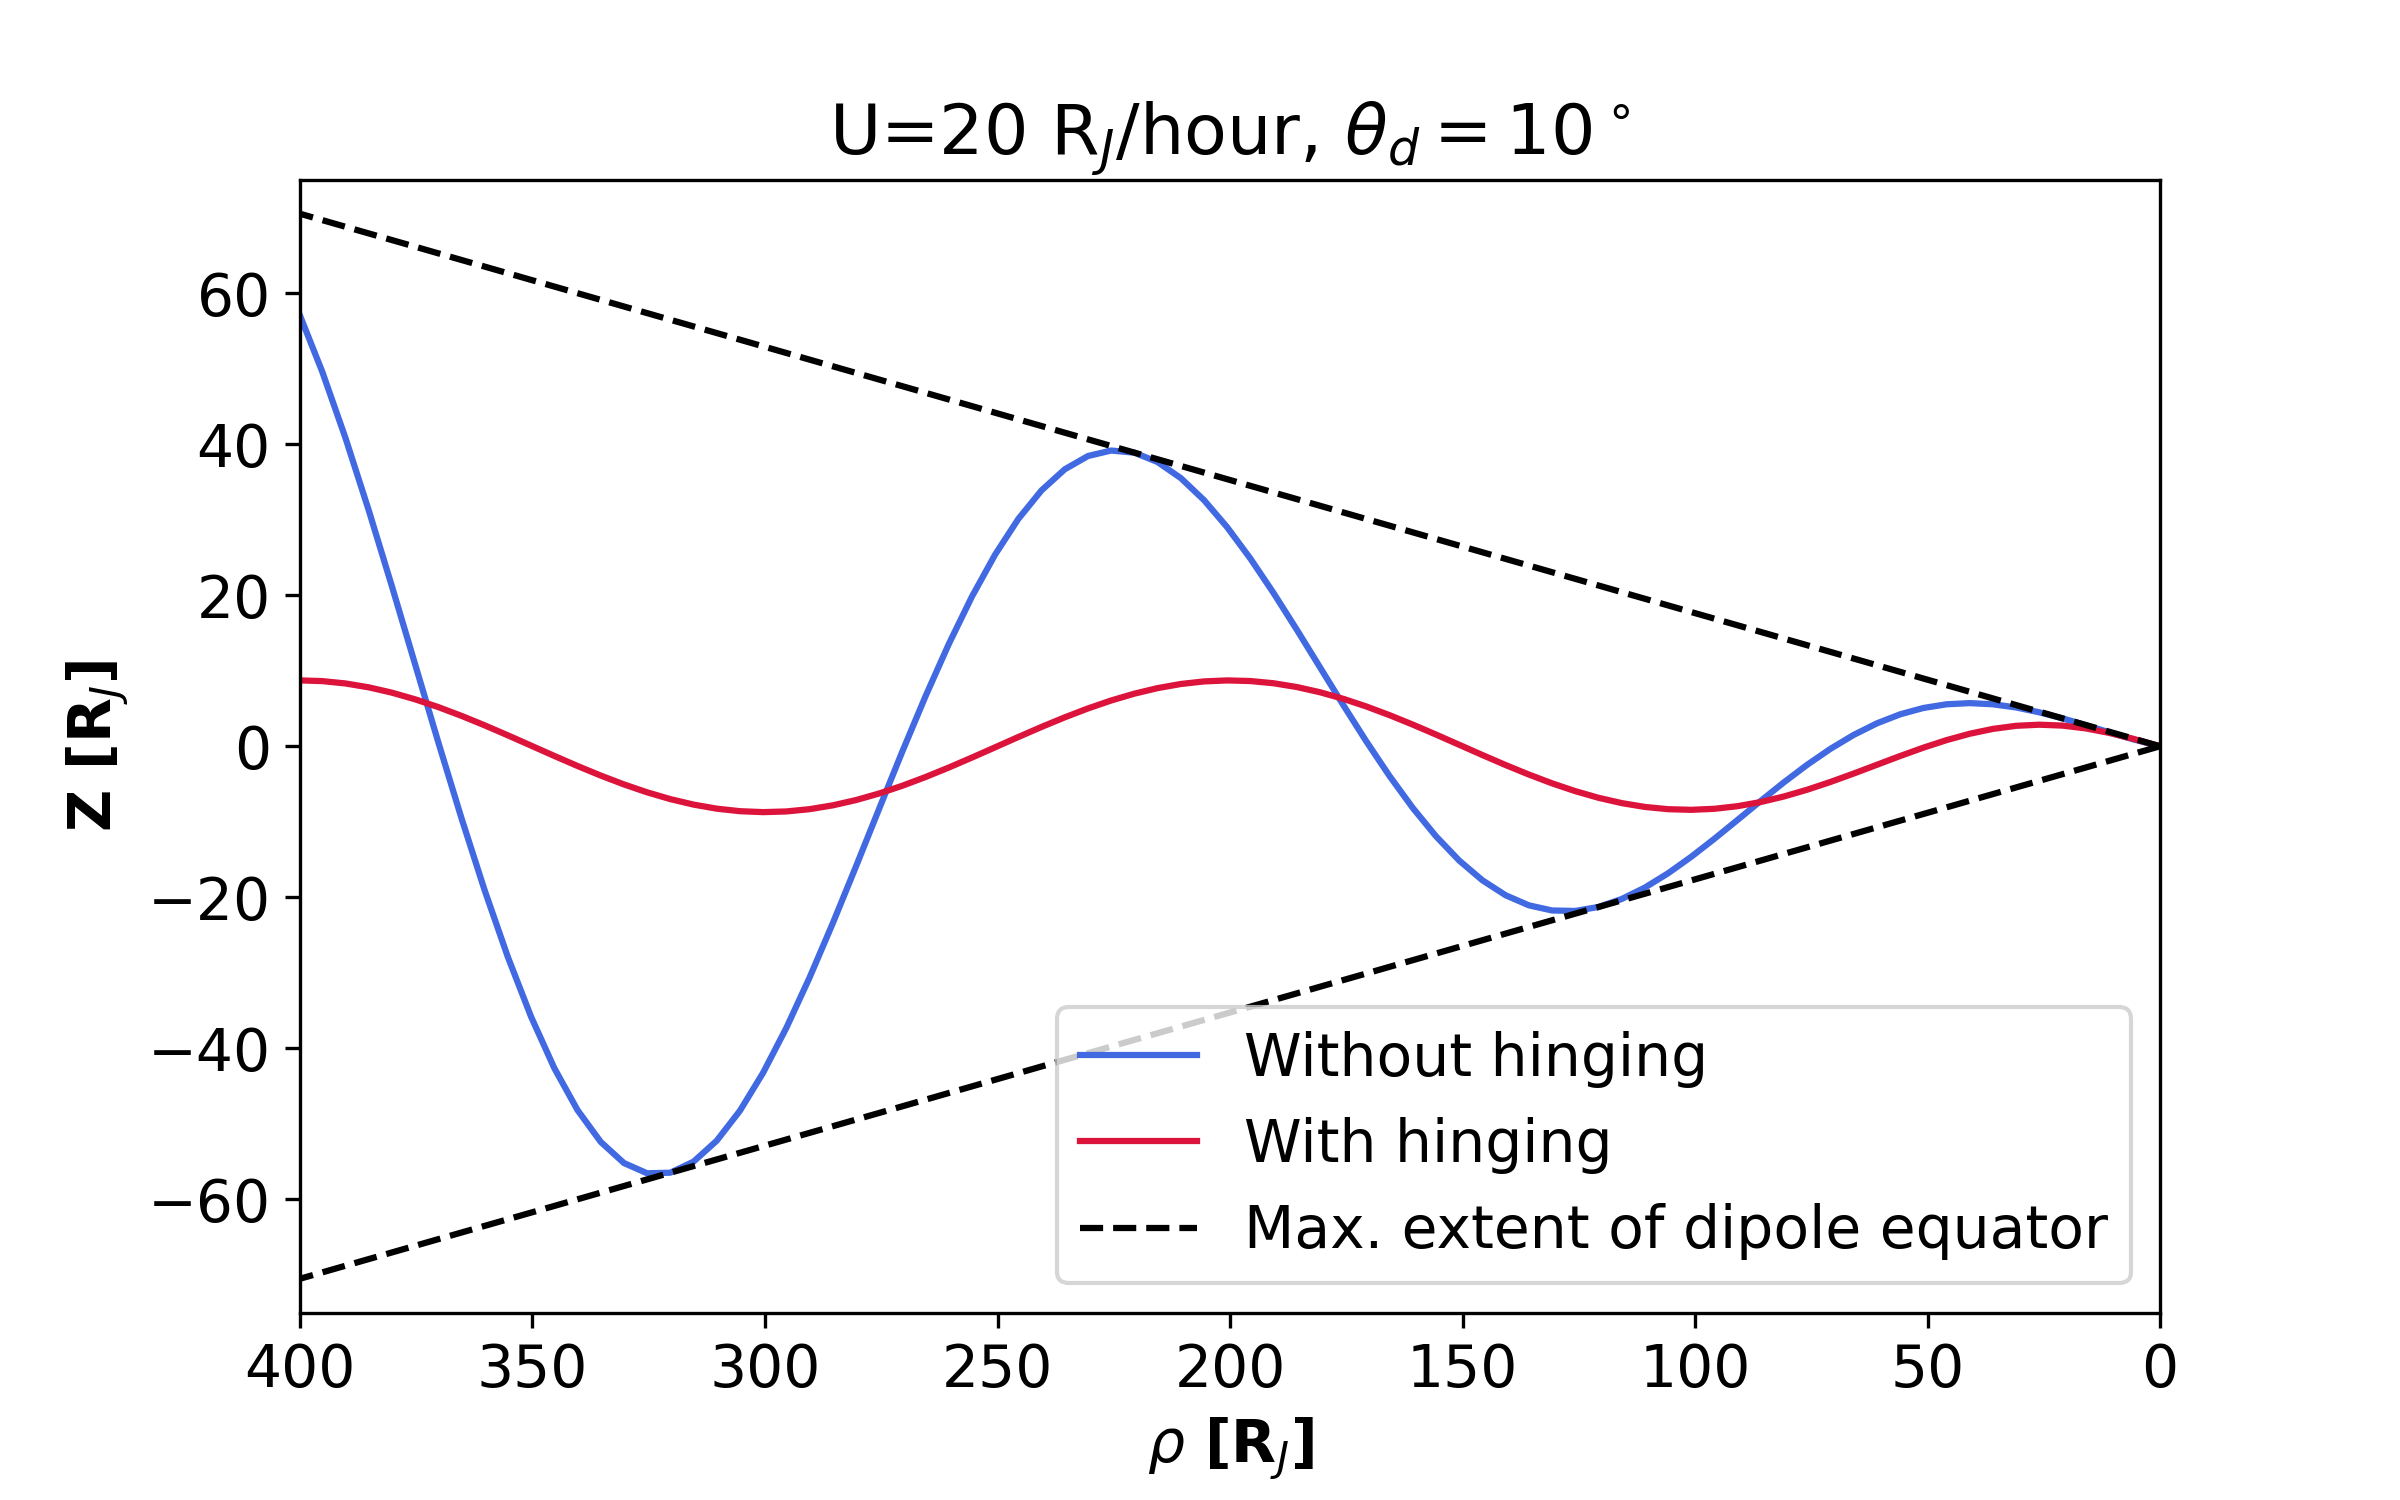
\includegraphics[width=0.8\textwidth]{images6/example-hinging.png}
    \caption{Examples of the Jovian current sheet locations for two different models. The \protect\citeA{Kivelson1978ASheet} model does not account for hinging of the current sheet and hence has larger excursions with increasing distance from the planet. The \protect\citeA{Behannon1981} model includes current sheet hinging, which limits the oscillations beyond a certain radial distance.}
    \label{fig:example-hinging}
\end{figure}

\section{MHD simulations with a tilted dipole}
To simulate the modulation of the Jovian current sheet, we modify the internal magnetic field of Jupiter to take the form of a dipole tilted 10$^\circ$ with respect to the spin axis and rotates around it at the planetary rotation period (10 hours). The simulations are performed in the GSE coordinate system. One change between the existing model and one described in Chapter 2 is the use of a cartesian grid instead of a spherical grid to avoid the ``pole-problem''. 

\section{Estimating the current sheet parameters within the MHD model}
As shown in Figure FIGURE, the current sheet location in our model varies with radial distance and dipole phase. A direct comparison between the current sheet location in the MHD model and the various empirical functions shows a poor fit, as small differences in phase can lead to large differences in the final current sheet location. Moreover, the empirical models have been observed to perform well only for the in-situ data to which they were originally fitted. For a more accurate comparison, we use the functional form for the various empirical models to find the set of parameters e.g. hinging distance, wave propagation speed, etc. which reproduce best the output seen in the MHD simulations.

We consider three models with relatively simple functional forms,
\begin{enumerate}
    \item The \citeA{Kivelson1978ASheet} model described by Equation \ref{eqn:kivelson1978} with two parameters - $U$ and $\rho_0$.
    \item The \citeA{Behannon1981} model described by Equation \ref{eqn:behannon1981} with two parameters - $U$ and $a_0$.
    \item The \citeA{Khurana1992ASheet} model described by Equation \ref{eqn:khurana1992} with three parameters - $v_0$, $x_0$ and $\rho_0$.
\end{enumerate}

The location of the current sheet is extracted in the noon-midnight meridian (00 LT) by identifying the locus of points located between $x=[-100, -4] R_J$ and $z=[-30, 30] R_J$ where  $B_r=0$. A current sheet model is then fitted to the extracted current sheet height $z_\text{MHD}$ at a given radial location $\rho$ by finding the set of parameters $\boldsymbol\theta$ that minimizes the square of the residual $\mathcal{R}$,

\begin{equation}
    \mathcal{R} = \sum_i^N \left[ z_\text{MHD}(\rho) - z_\text{fit} (\rho, \boldsymbol\theta) \right]_i^2
\end{equation}

The Nelder-Mead iterative algorithm is used to perform the non-linear minimization. We repeat the above procedure for all simulation data files separated by an interval of 30 minutes, giving us 200 data points within a 100 hour interval for each model. Although we limit our analysis to regions in the $y=0$ plane and $x < -4 R_J$ (nightside magnetotail), we effectively sample different phases of the current sheet due to the rotation of the dipole every 10 hours.

\begin{figure}
    \centering
    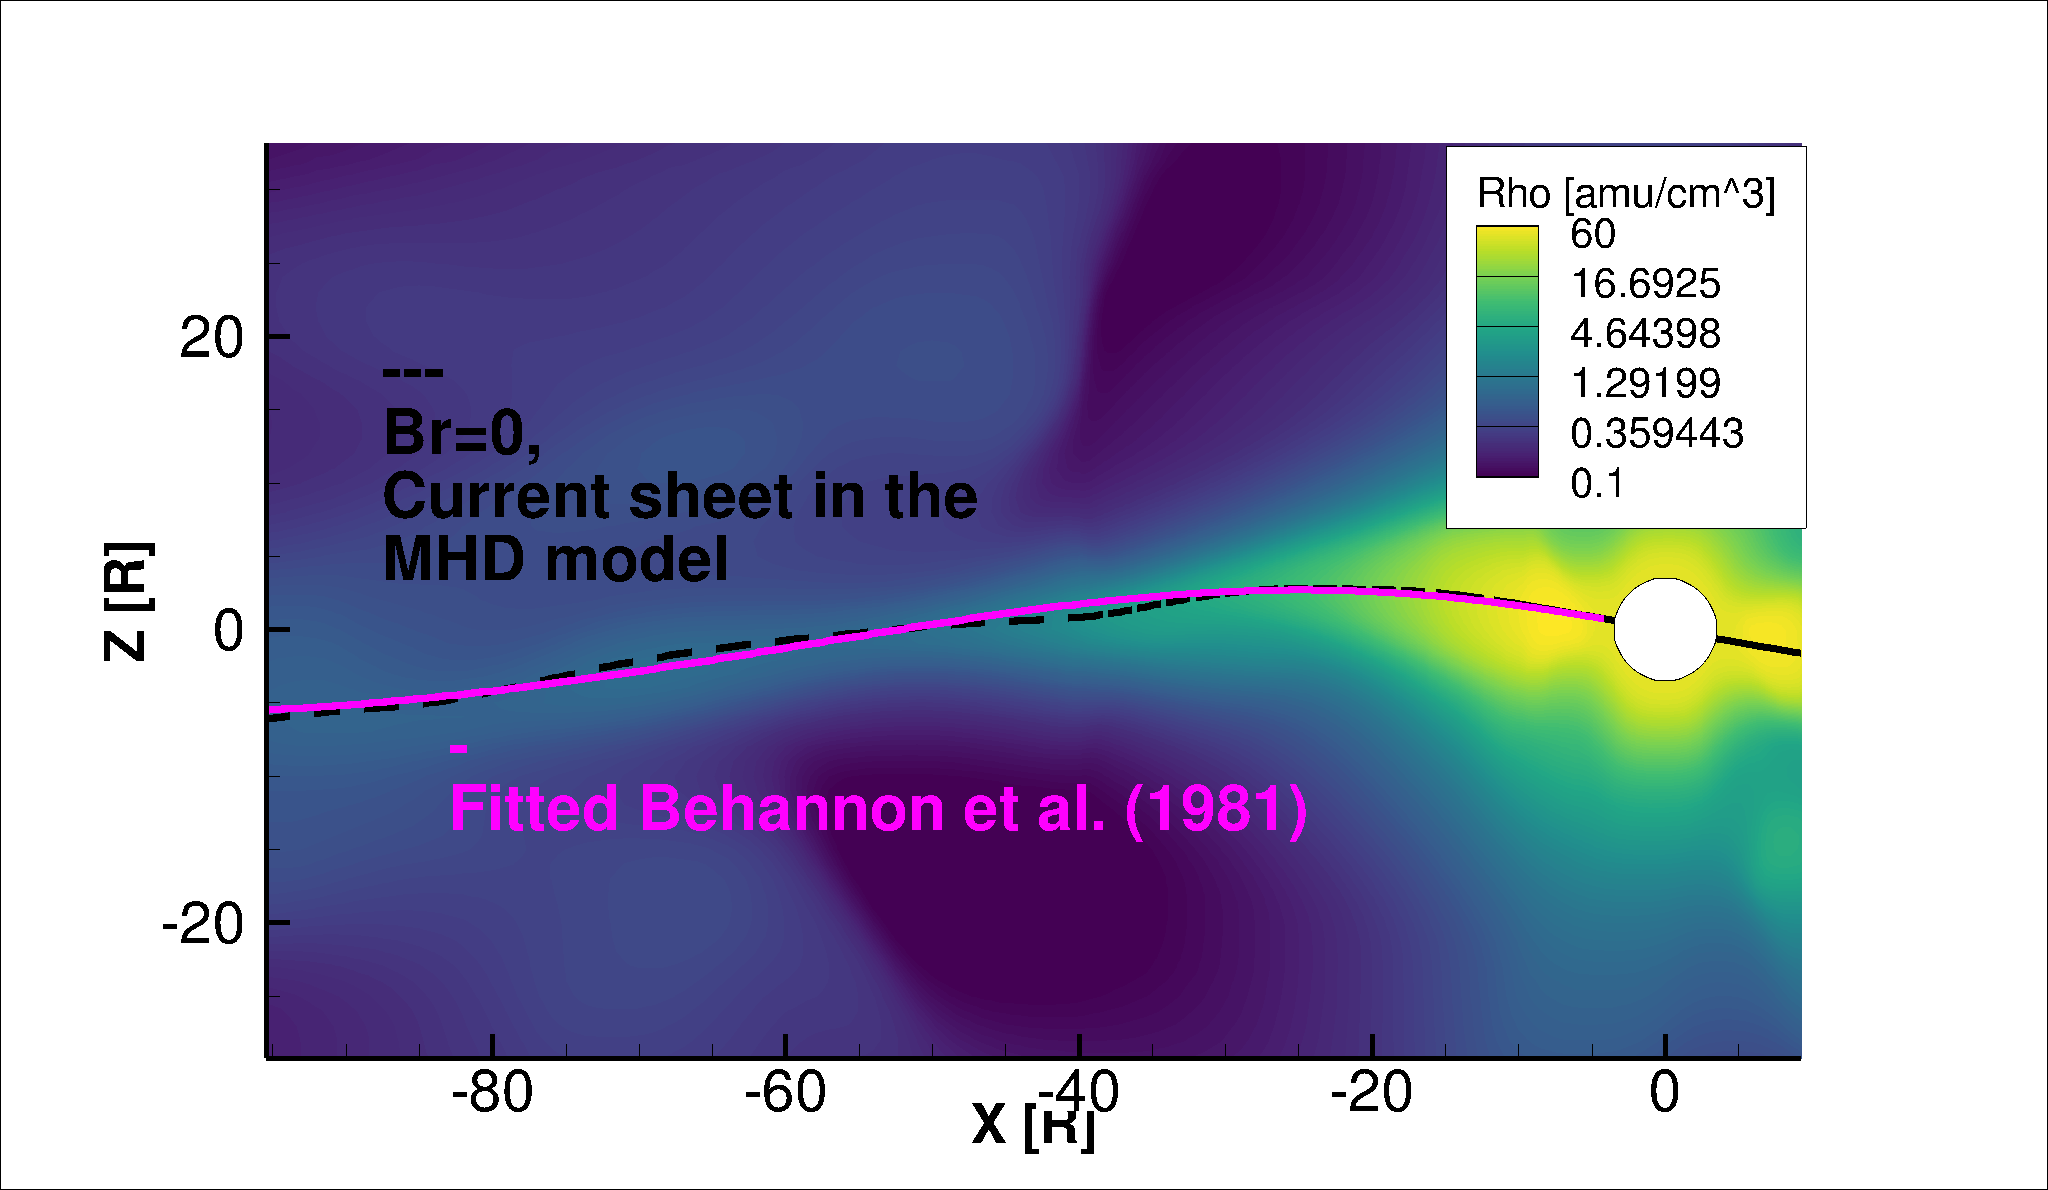
\includegraphics[width=\textwidth]{images6/CurrentSheet_fitted.png}
    \caption{Caption}
    \label{fig:example-fitcurrentsheet}
\end{figure}

Figure \ref{fig:example-fitcurrentsheet} shows the result of fitting the \citeA{Behannon1981} model for the current sheet to that observed at that instance in the MHD simulations. In this instance, the wave velocity $U$ and the hinging distance $a_0$ are estimated to be <> $R_J$/hour and <> $R_J$ respectively. 

\section{Variation of current sheet parameters with solar wind dynamic pressure}

\begin{figure}
    \centering
    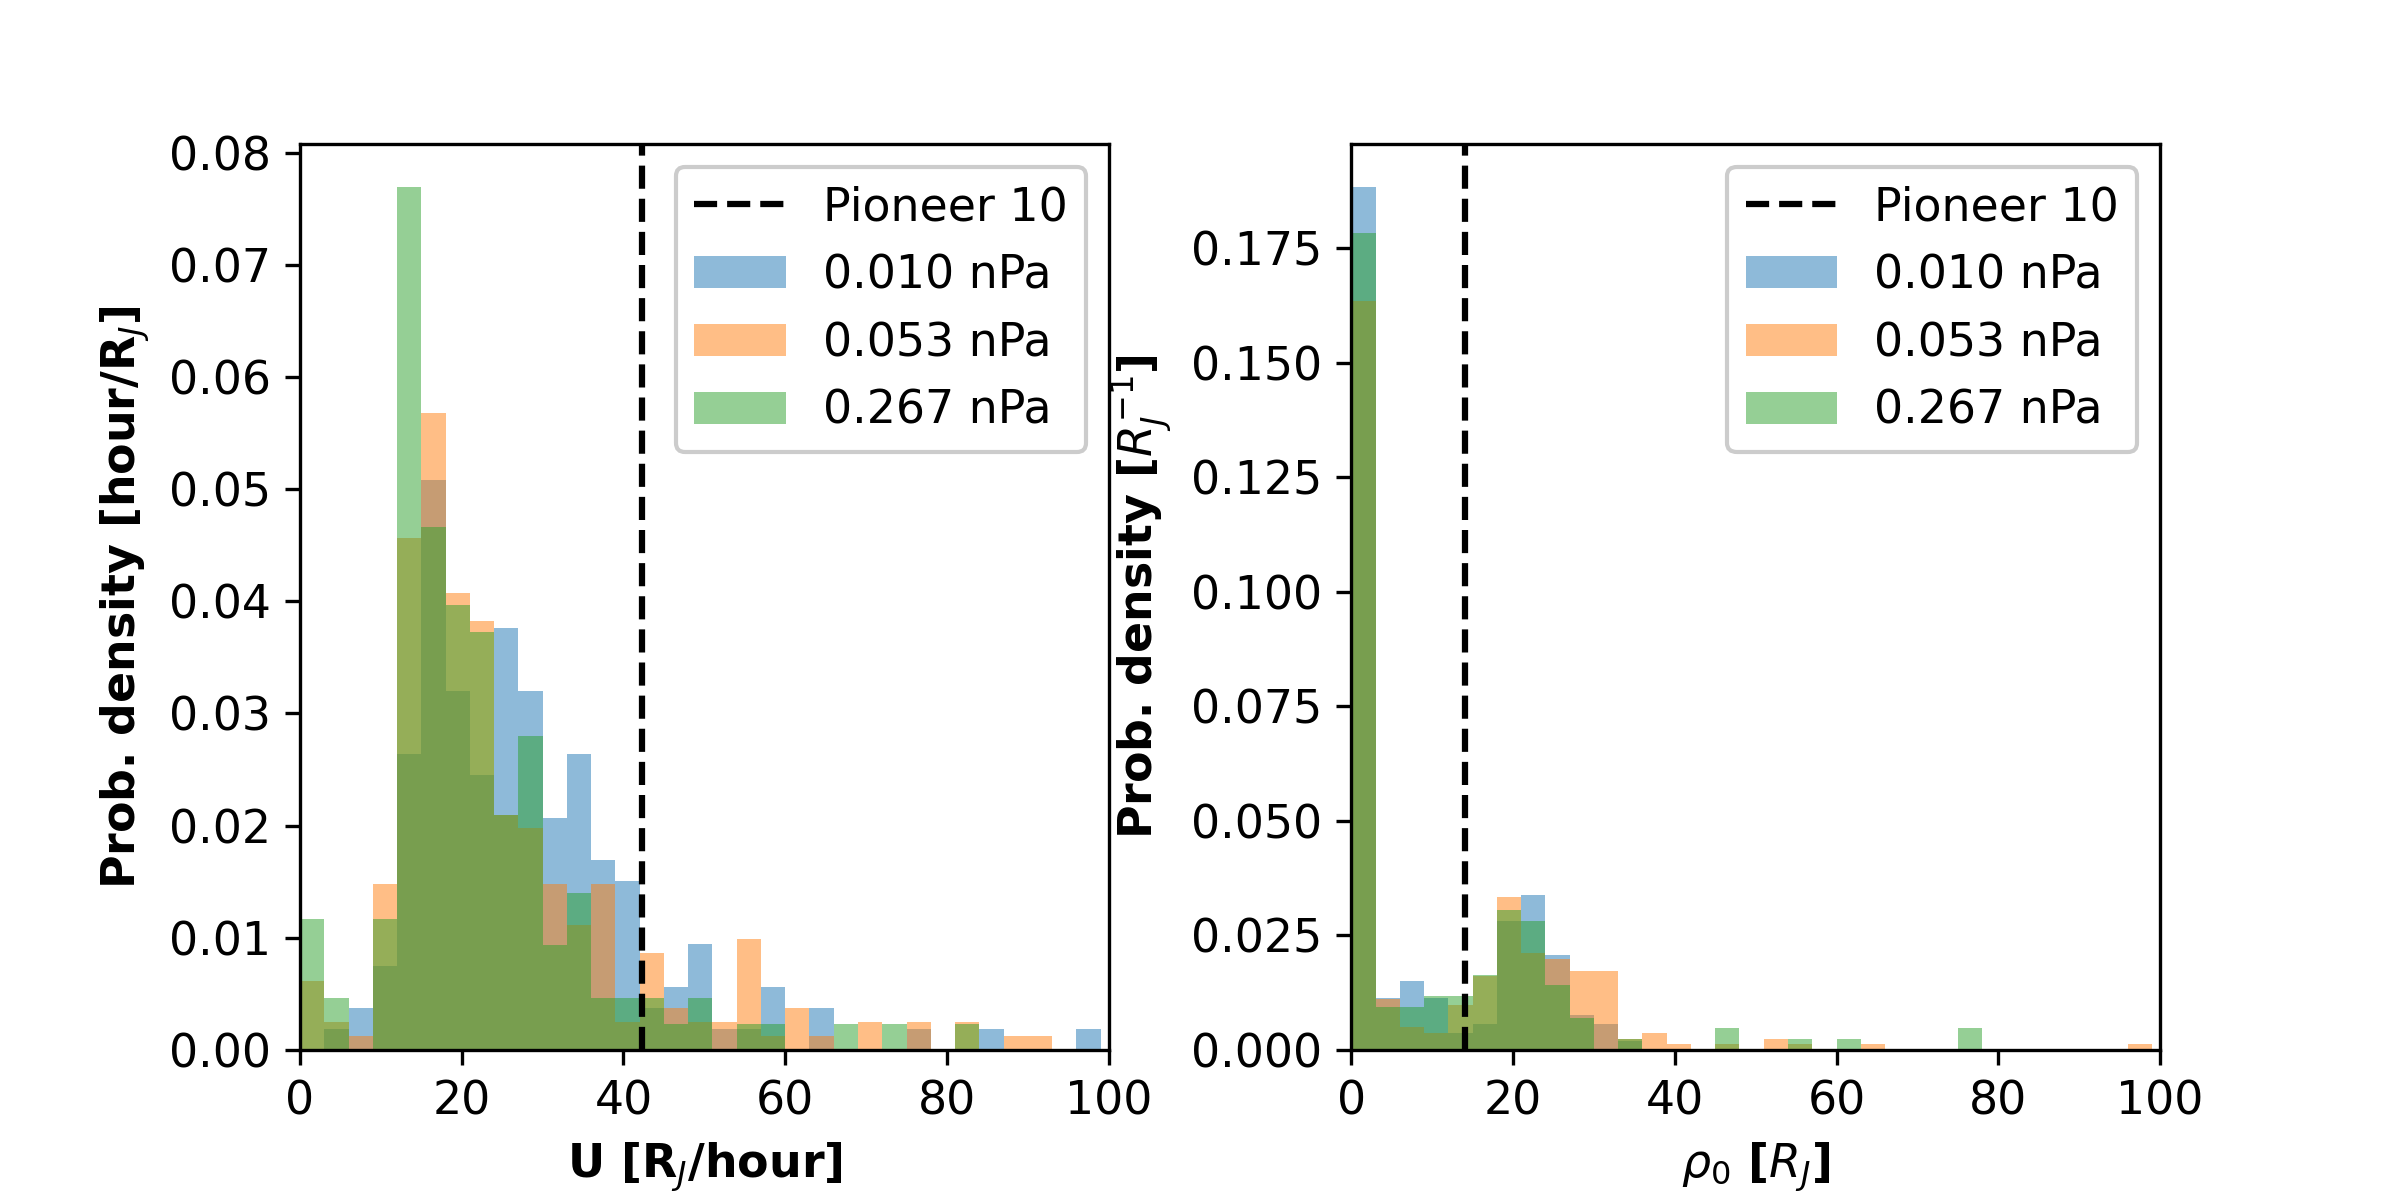
\includegraphics[width=\textwidth]{images6/comparison_highdynP_kivelson.png}
    \caption{Caption}
    \label{fig:comparison-hist-kivelson}
\end{figure}

\begin{figure}
    \centering
    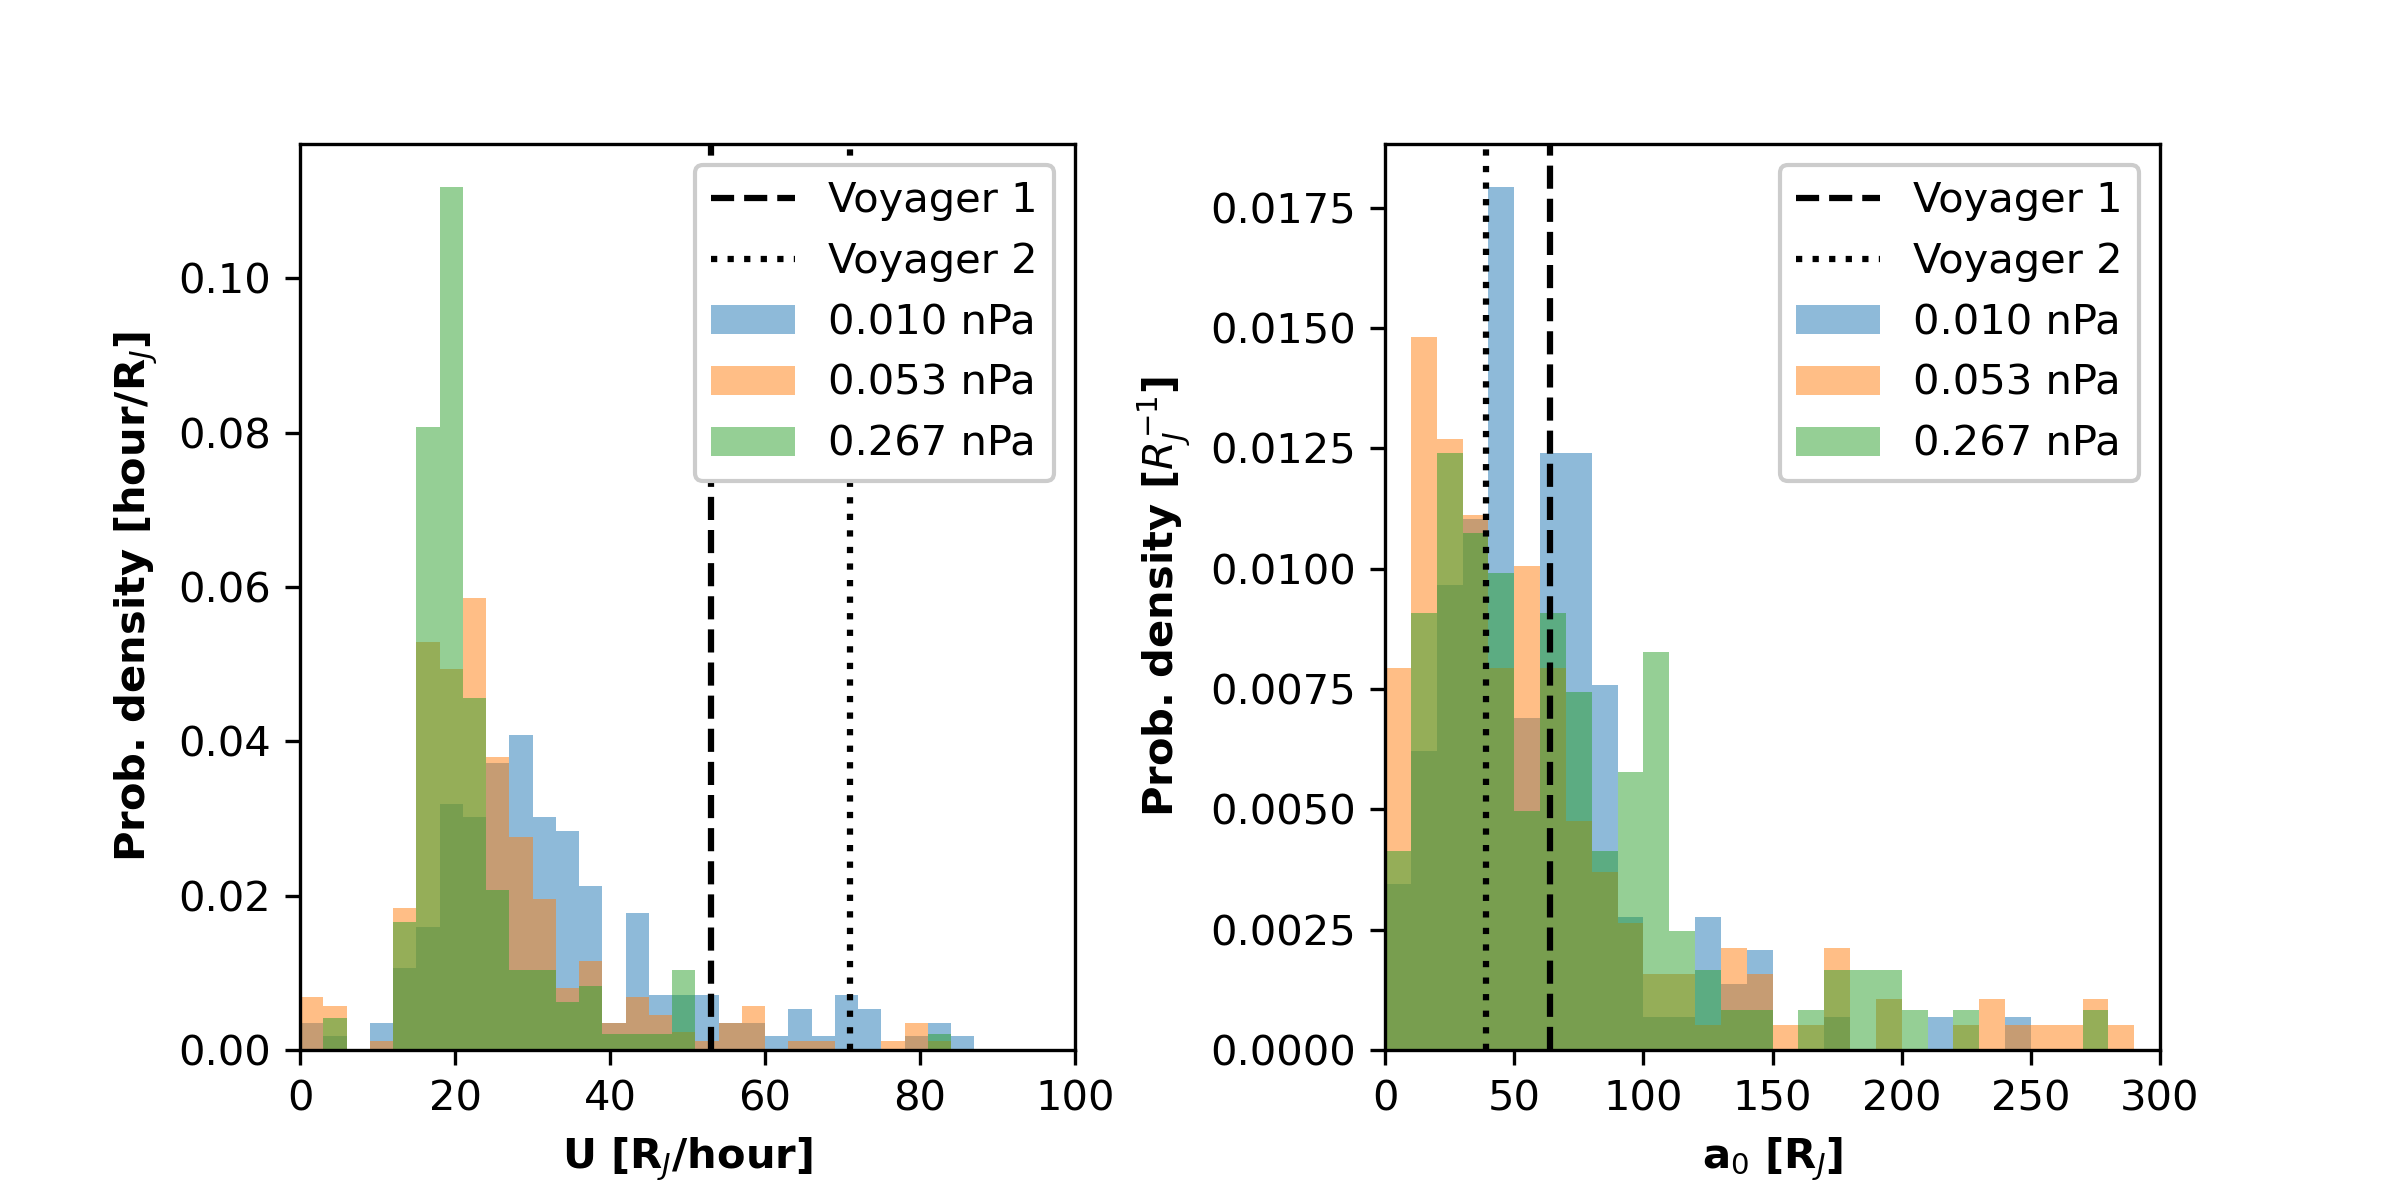
\includegraphics[width=\textwidth]{images6/comparison_highdynP_behannon.png}
    \caption{Caption}
    \label{fig:comparison-hist-behannon}
\end{figure}

\begin{figure}
    \centering
    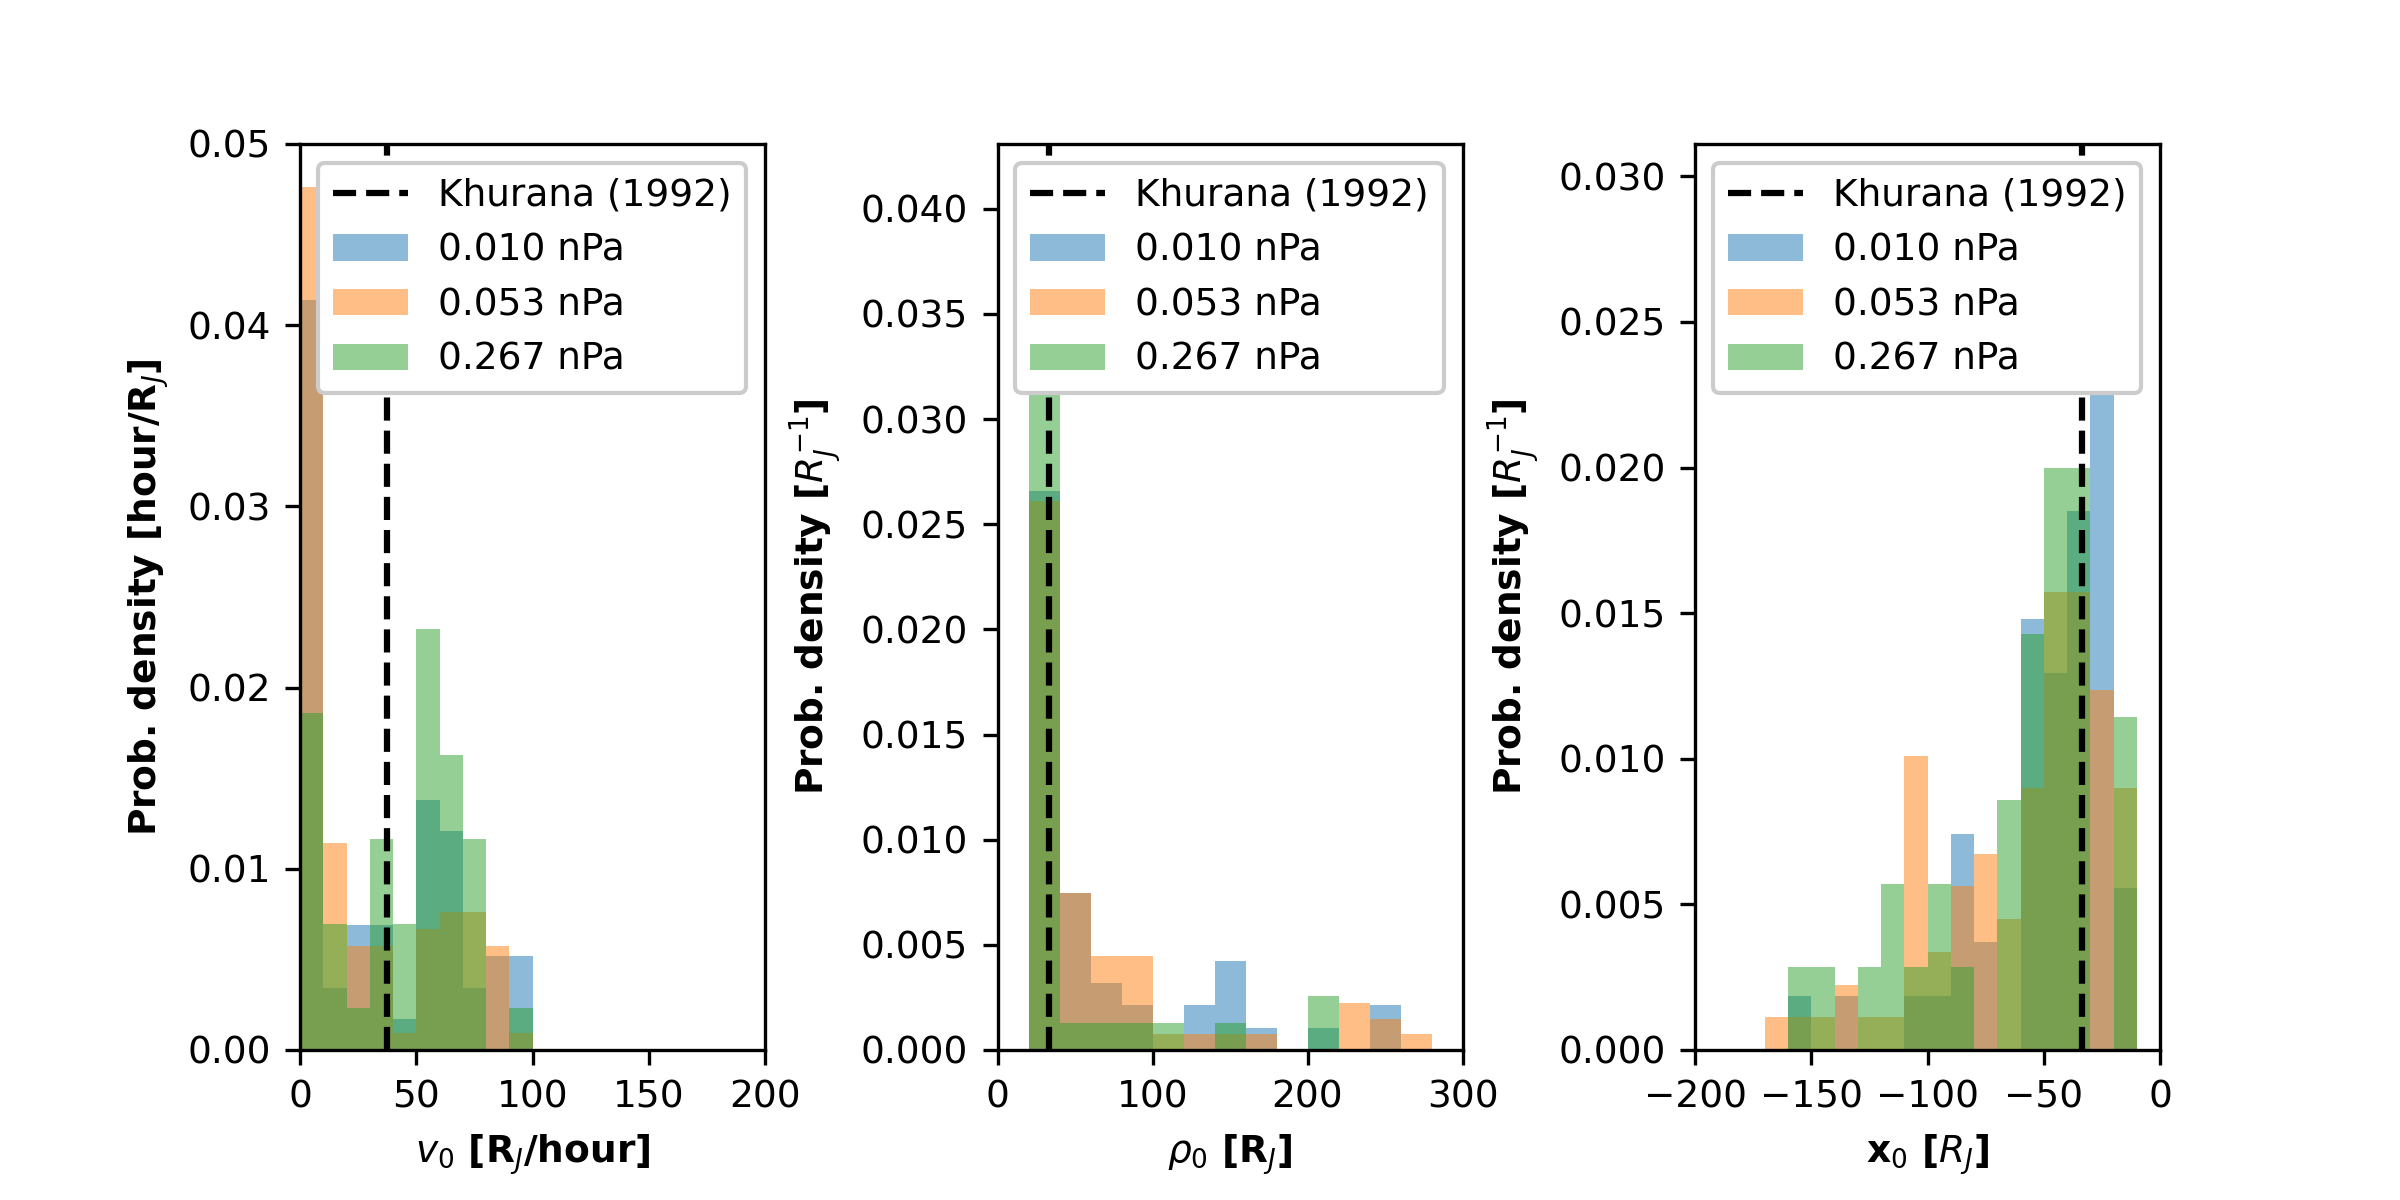
\includegraphics[width=\textwidth]{images6/comparison_highdynP_khurana.png}
    \caption{Caption}
    \label{fig:comparison-hist-khurana}
\end{figure}


\section{Discussion}